\section{Introduction}
\label{sec:intro}

A learned codec normally spends the same synthesis computation on every
part of an image. Yet another pair of decoder blocks may recover visible
structure in one region and change almost nothing in its neighbour.
Making each block faster lowers the cost of both regions; deciding
\emph{where the blocks run} addresses a different inefficiency. This is
the question behind \textbf{RegLIC}: can a codec allocate reconstruction
capacity locally without giving up the compression benefits of a shared
representation?

\begin{figure}[t]
\centering
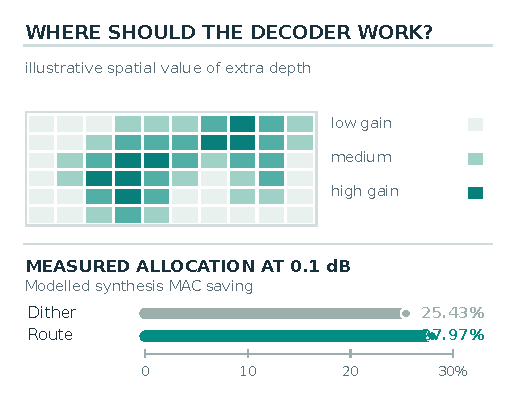
\includegraphics[width=\columnwidth]{figs/reglic_intro/reglic_intro.pdf}
\caption{\textbf{Depth is a spatial decision.} \textbf{Top:} a schematic
tile field illustrates that the value of additional synthesis can vary
within one image; colours are conceptual, not measured tile errors.
\textbf{Bottom:} at a nominal 0.1\,dB $\Delta_{444}$ target, learned
routing saves \MainRouterSaving\% of \emph{modelled synthesis MACs},
versus \MainDitherSaving\% for ordered dithering
(\MainPremium{}-point difference). These source-calibrated results are
not end-to-end latency measurements.}
\label{fig:intro}
\end{figure}

Spatial capacity selection is established in restoration: ClassSR
assigns super-resolution patches to networks of different sizes
\cite{kong2021classsr}, while APE lets patches leave a shared network
according to predicted incremental benefit~\cite{wang2022ape}.
AdaNIC brings spatially dynamic transforms to image compression
\cite{tao2023adanic}. For a codec, however, decoder depth is coupled to
the coded representation and the rate at which it was produced. A
visually complex patch need not benefit from a deeper decoder if its
bitstream carries little recoverable detail. The relevant quantity is
therefore the \emph{marginal reconstruction gain} of more synthesis,
relative to its computation and coding cost.

We study this allocation in the intra model of DCVC-UF
\cite{li2026dcvcuf}. Its twelve constant-width synthesis blocks expose
depth as a clean capacity axis without changing feature width. RegLIC
has two complementary realisations. In the
\emph{shared-exit} path, every region uses the same coded latent and
decoder prefix, then exits after a chosen block pair. In the
\emph{independent-depth} path, a selector chooses a complete 2/4/6/8/10/12-
block codec before encoding a region, allowing its analysis and entropy
models to specialise as well. The latter trades representation reuse
for specialised coding and introduces region-boundary and signalling
costs. We evaluate the shared-exit path here; the independently trained
bank is an ongoing capacity study, not a demonstrated routed system.

The evaluated design must actually \emph{skip} computation: computing
every depth and choosing an output afterwards would save no decoding
work. A full-frame stem supplies a common latent feature canvas;
conditional block pairs process a shrinking batch of active tiles.
Exit adapters align features from different depths before a shared
full-frame repair and reconstruction head. This preserves a common
output path while allowing each tile to stop at a different depth.

Separating the benefit of shallow decoding from the benefit of
\emph{placing} deeper computation is central to the evaluation.
Uniform exits and ordered dithering already reduce average depth;
the latter mixes depths without predicting which locations need them.
At a nominal 0.1\,dB YCbCr-MSE-ratio target across 53 intra frames and
five QPs, routing saves \MainRouterSaving\% of modelled synthesis MACs,
\MainPremium\ percentage points more than dithering under
per-source calibration (\cref{fig:intro}). A retrospective common
delivered-loss cap retains a margin, but when controls are fitted on
other sequences, the QP32 paired advantage is unresolved. The
arithmetic saving is consequently established more strongly than a
source-independent routing gain or complete-codec speedup.

Our contributions are a conditional DCVC-UF synthesis path with
executed tile exits; a controlled comparison that isolates spatial
placement from cheaper average depth; and a depth-bank protocol that
tests the separate question of whether independent representation
specialisation can repay its coding and boundary costs. Together they
turn synthesis depth from a fixed architectural choice into an
explicit, measurable spatial allocation problem.
